\documentclass[a4paper,12pt]{article}
%%%%%%%%%%%%%%%%%%%%%%%%%%%%%%%%%%%%%%%%%%%%%%%%%%%%%%%%%%%%%%%%%%%%%%%%%%%%%%%%%%%%%%%%%%%%%%%%%%%%%%%%%%%%%%%%%%%%%%%%%%%%%%%%%%%%%%%%%%%%%%%%%%%%%%%%%%%%%%%%%%%%%%%%%%%%%%%%%%%%%%%%%%%%%%%%%%%%%%%%%%%%%%%%%%%%%%%%%%%%%%%%%%%%%%%%%%%%%%%%%%%%%%%%%%%%
\usepackage{eurosym}
\usepackage{vmargin}
\usepackage{amsmath}
\usepackage{graphics}
\usepackage{epsfig}
\usepackage{subfigure}
\usepackage{fancyhdr}
\usepackage{listings}
\usepackage{framed}
\usepackage{graphicx}
\usepackage{amsmath}
\usepackage{chngpage}
%\usepackage{bigints}


\setcounter{MaxMatrixCols}{10}

\begin{document}
	\large
%%- http://dev.socrata.com/consumers/examples/data-visualization-with-python.html

%==================================%


\begin{figure}[h!]
\centering
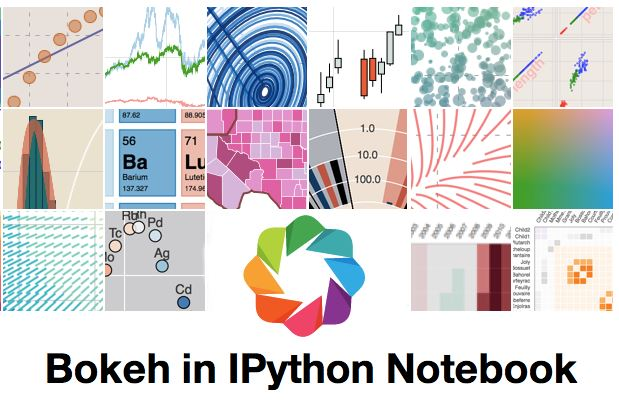
\includegraphics[width=0.9\linewidth]{images/TitleSlide}
\end{figure}

\begin{quote}
Bokeh is a Python interactive visualization library for large datasets that natively uses the latest web technologies. Its goal is to provide elegant, concise construction of novel 
graphics in the style of Protovis/D3, while delivering high-performance interactivity over large data to thin clients.

\end{quote}
\newpage
\begin{itemize}
\item Bokeh is developed by \textbf{Continuum Analytics}.
\end{itemize}
\begin{figure}[h!]
\centering

\includegraphics[width=1.0\linewidth]{images/continuum}
\end{figure}

\begin{figure}[h!]
\centering
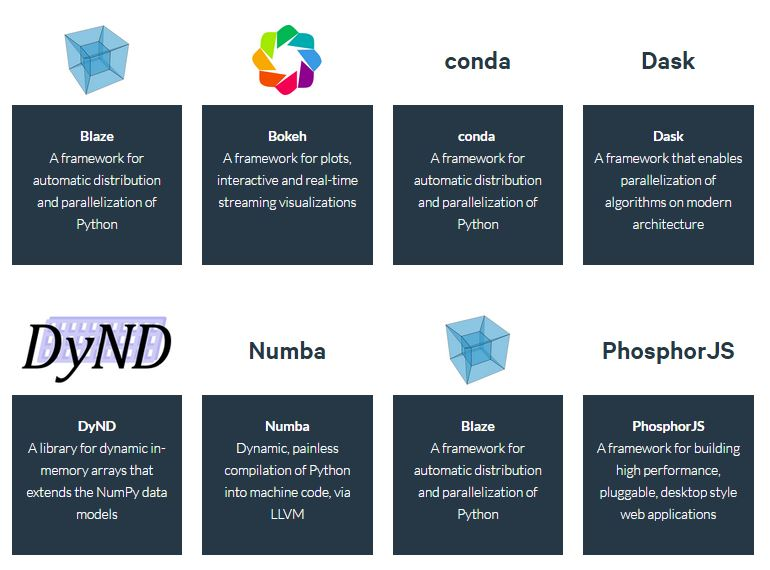
\includegraphics[width=0.9\linewidth]{images/00-continuum-projects}
\end{figure}
\newpage
\section*{Bokeh scales visualization to Big Data}
\textit{(From Bokeh Documentation)}
\begin{itemize}
\item Interactive and real-time streaming visualization framework that scales to Big Data with data shading

\item Bokeh is a Python data visualization library combining the ideas of the \textbf{Grammar of Graphics} and \textbf{Protovis}, with enhancements to support interactive visualization. Its primary output backend is HTML5 Canvas.

\item There are many excellent plotting packages for Python, but they generally do not optimize for the particular needs of statistical plotting or multidimensional datasets. 
\item Additionally, advanced visual customization is typically difficult for non-programmers, and most libraries do not build a reified data processing pipeline that supports rich interactivity like linked brushing. 
\item Bokeh addresses these problems at their core by using a declarative data transformation scheme, and is engineered to operate in a client/server model for the modern web.


\item Bokeh can produce elegant and interactive visualization like D3.js with high-performance interactivity over very large or streaming datasets. Bokeh can help anyone who would like to quickly and easily create interactive plots, dashboards, and data applications.
\end{itemize}

\newpage
%==================================%
\begin{framed}
	\noindent \textbf{Benefits of Bokeh:}
	
	\begin{itemize}
		\item Bokeh allows you to build complex statistical plots quickly and through simple commands
		\item Bokeh provides you output in various medium like html, notebook and server
		\item We can also embed Bokeh visualization to flask and django app
		\item Bokeh can transform visualization written in other libraries like matplotlib, seaborn, ggplot
		\item Bokeh has flexibility for applying interaction, layouts and different styling option to visualization
	\end{itemize}
\end{framed}
%==================================%
\newpage
\subsection*{Installation}
You may need to install a few Python packages :


\begin{framed}
\begin{verbatim}
conda install pandas
conda install bokeh
\end{verbatim}
\end{framed}

\subsection*{IMPORTANT : Version}

\begin{figure}[h!]
\centering
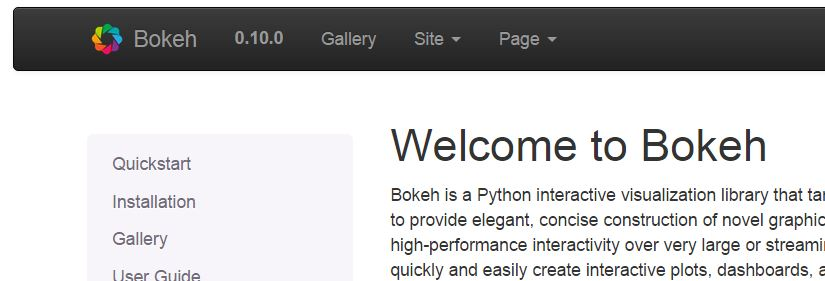
\includegraphics[width=0.7\linewidth]{images/00-BOKEH-version}
\end{figure}
\begin{itemize}
\item This workshop will be based on version 0.10. 
\item A lot of code for older version of Bokeh no longer work.
\item To check what version you actually have installed, run the following code
\end{itemize}


\begin{figure}[h!]
	\centering
	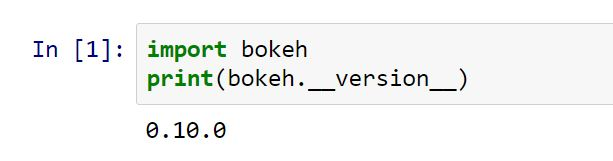
\includegraphics[width=0.9\linewidth]{images/00-BOKEH-version-check}
\end{figure}
%==================================%
\newpage
\begin{framed}
	\noindent \textbf{Challenges with Bokeh}
	\begin{itemize}
		\item Like with any upcoming open source library, Bokeh is undergoing a lot of development. So, the code you write today may not be entirely reusable in future.
		
		\item  It has relatively less visualization options, when compared to \textbf{\textit{D3.js}}. Hence, it is unlikely in near future that it will challenge \textbf{\textit{D3.js}} for its crown.
		\item  Given the benefits and the challenges, it is currently ideal to rapidly develop prototypes. However, if you want to create something for production environment, \textbf{\textit{D3.js}} might still be your best bet.
	\end{itemize}
\end{framed}
\newpage
\section*{Bokeh Graphics with Jupyter Notebooks}

\begin{framed}
\noindent \textbf{Displaying Inline Plots}\\ 
To display Bokeh plots inline in an IPython/Jupyter notebook, use the \texttt{output\_notebook()} function from bokeh.io instead of (or in addition to) the \texttt{output\_file()}
\end{framed}

\begin{itemize}
	\item Open up a Jupyter Notebook, and enter the following code in over three or four cells.
	\item Run those cells. The output should come up on a new HTML page. (See next page).
	\item The output graphic has some controls (pan , zoom, resize etc). Try these controls out.
	\item Vary some of the values (width, either , title).
\end{itemize}
\begin{framed}
	\begin{verbatim}
	#Import library
	from bokeh.charts import Bar, output_file, show 
	
	
	#use output_file to visualize it in html file
	#use output_notebook to visualize it in notebook
	
	# create a simple data set
	myData = {"y": [1, 2, 3, 4, 5]}
	
	# Output to Line.HTML
	output_file("lines.html", title="line plot example") 
	
	# create a new line chat with a title and axis labels
	p = Bar(myData, title="Simple Bar Chart Example",
	label='x', ylabel='values', 
	width=400, height=400)
	
	# show the results
	show(p)
	
	\end{verbatim}
\end{framed}
\newpage
\begin{figure}[h!]
	\centering
	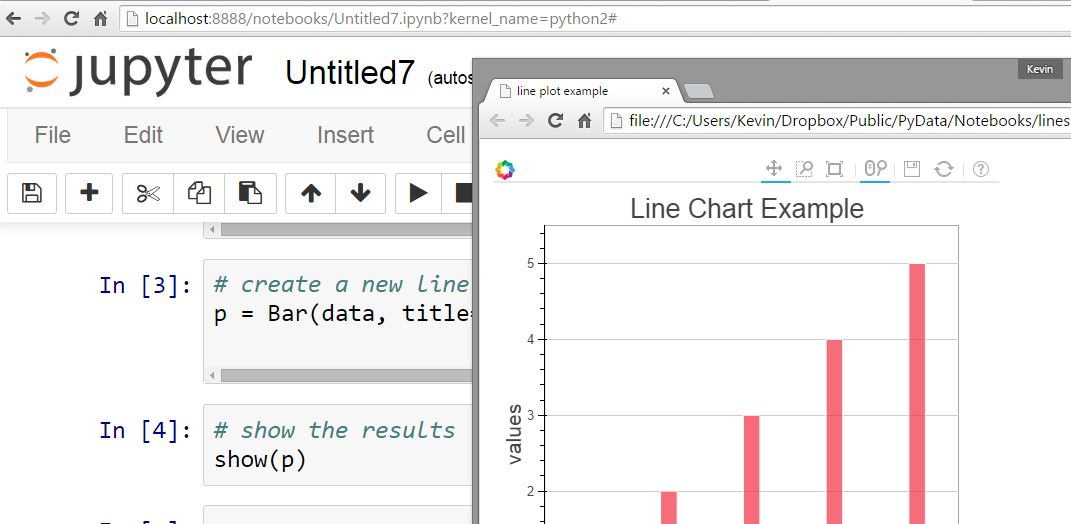
\includegraphics[width=0.9\linewidth]{images/OutPut}
	\caption{Output}\vspace{0.5cm}
	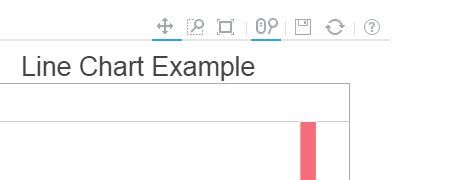
\includegraphics[width=0.8\linewidth]{images/TopRightCorner}
	\caption{Controls}
\end{figure}
\newpage
%==================================%
\section*{Visualization with Bokeh}
\begin{itemize}
	\item Bokeh offers both powerful and flexible features which imparts simplicity and highly advanced customization. 
	
	
	
	\item It provides multiple visualization interfaces to the user as shown below:\texttt{Bokeh\_Interface}
\end{itemize}



\begin{description}
	\item[Charts:] a high-level interface that is used to build complex statistical plots as quickly and in a simplistic manner.
	\item[Plotting:] an intermediate-level interface that is centered around composing visual glyphs.
	\item[Models:] a low-level interface that provides the maximum flexibility to application developers.
\end{description}
%In this article, we will look at first two interfaces charts and plotting only. 
%
%We will discuss models and other advance feature of this library in next post.


%========================================================================% 
\newpage

\section*{Charts Example 1}

As mentioned above, it is a high level interface used to present information in standard visualization form. 
These forms include box plot, bar chart, area plot, heat map, donut chart and many others. You can generate these plots just by passing data frames, numpy arrays and dictionaries.

Let’s look at the common methodology to create a chart:

\begin{itemize}
	\item Import the library and functions/ methods
	\item Prepare the data
	\item Set the output mode (Notebook, Web Browser or Server)
	\item Create chart with styling option (if required)
	\item Visualize the chart
\end{itemize}

%\newpage
%
%To understand these steps better, let me demonstrate these steps using example below:
%
%Charts Example-1: 
%
%Create a bar chart and visualize it on web browser using Bokeh
%
%We will follow above listed steps to create a chart:

\newpage

\begin{verbatim}
#Import library

from bokeh.charts import Bar, output_file, show 
#use output_notebook to visualize it in notebook

# prepare data (dummy data)
data = {"y": [1, 2, 3, 4, 5]}

# Output to Line.HTML
output_file("lines.html", title="line plot example") 

#put output_notebook() for notebook

# create a new line chat with a title and axis labels
p = Bar(data, title="Line Chart Example", xlabel='x', 
ylabel='values', width=400, height=400)

# show the results
show(p)
\end{verbatim}

\newpage
\begin{itemize}
	\item \textbf{Important:} In the chart above,  you can see the tools at the top (zoom, resize, reset, wheel zoom) and these 
	tools allows you to interact with chart. 
	\item You can also look at the multiple chart options (legend, xlabel, ylabel, xgrid, width, height and many other) and 
	various example of charts here.
\end{itemize}



%========================================================================% 

\section*{Charts Example 2}
\begin{itemize}
	\item Compare the distribution of sepal length and petal length of IRIS data set using 
	Box plot on notebook
	
	\item To create this visualization, we can import the iris data set using \textbf{\textit{sklearn library}}. 
	\item Then, 
	follow the steps as discussed above to visualize chart in ipython notebook.
	
\end{itemize}

\newpage


\begin{verbatim}
#IRIS Data Set

from sklearn.datasets import load_iris
import pandas as pd
iris = load_iris()

df=pd.DataFrame(iris.data)
df.columns=['petal_width','petal_length',
'sepal_width','sepal_length']

#Import library
from bokeh.charts import BoxPlot,   
output_notebook, show
data=df[['petal_length','sepal_length']]

# Output to Notebook
output_notebook()

# create a new line chat with a title and axis labels
p = BoxPlot(data, width=400, height=400)

# show the results
show(p)
Bokeh_Box_Plot
\end{verbatim}

%========================================================================%

\section*{Components}
\Large

Bokeh is actually composed of two library components.

\begin{itemize}
	\item The first component is a JavaScript library, \texttt{BokehJS}, that runs in the browser. This library is responsible for all of the rendering and user interaction. Its input is a collection of declarative JSON objects that comprise a “scenegraph”. 
	\item The objects in this scenegraph describe everything that BokehJS should handle: what plots and widgets are present and in what arrangement, what tools and renderers and axes the plots will have, etc. These JSON objects are converted into Backbone Models in the browser, and are rendered by corresponding Backbone Views.
	
	\item The second component is a library in Python (or other languages) that can generate the JSON described above. In the Python Bokeh library, this is accomplished at the lowest level by exposing a set of “model” classes that exactly mirror the set of Backbone Models that are created in the browser. 
	\item These python model classes know how to validate their content and attributes, and also how to serialize themselves to JSON. 
	
\end{itemize}
\newpage
\section*{Interfaces}
\begin{figure}[h!]
	\centering
	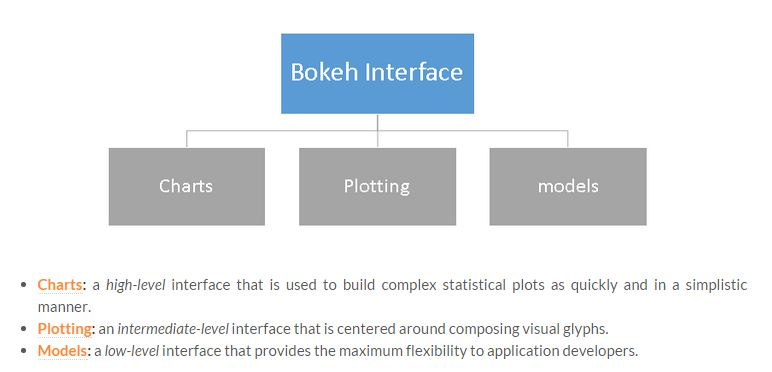
\includegraphics[width=1.1\linewidth]{images/00-Interfaces}
\end{figure}
\begin{itemize}
	\item Bokeh is intended to be useful to data-scientists and domain experts, working at a very high level, as well as to application developers and software engineers, who may want more control or access to more sophisticated features. 
	\item Because of this, Bokeh takes a layered approach and offers programming interfaces appropriate to different levels, as well as some compatibility interfaces to make use of existing code from other libraries. 
	
	\item This section provides an overview of the different interfaces that are available to Bokeh users, as well as more context about the most important concepts central to the library. 
	% If you’d like to jump right into plotting, go to Plotting with Basic Glyphs or Using High-level Charts.
\end{itemize}



%===================================================================================== %
\newpage

\section*{\texttt{bokeh.models}}

\begin{itemize}
	\item All of the \textbf{\textit{low level}} models live in the low-level \texttt{bokeh.models} interface. \item Most of the models are very simple, usually consisting of a few property attributes and no methods. 
	\item Model attributes can either be configured when the model is created, or later by setting attribute values on the model object. 
	
\end{itemize}

Here are some examples for a \texttt{Rect glyph} object:

\begin{framed}
	\begin{verbatim}
	
	# properties can be configured when a 
	# model object is initialized
	glyph = Rect(x="x", y="y2", 
	w=10, h=20, line_color=None)
	
	# or by assigning values to attributes
	# on the model later
	glyph.fill_alpha = 0.5
	glyph.fill_color = "navy"
	\end{verbatim}
\end{framed}
\newpage
\begin{itemize}
	\item These methods of configuration work in general for all Bokeh models. Because of that, and because all Bokeh interfaces ultimately produce collections of Bokeh models, styling and configuring plots and widgets is accomplished in basically the same way, regardless of which interface is used.
	
	\item Using the \texttt{bokeh.models} interface provides complete control over how Bokeh plots and Bokeh widgets are put together and configured.\\ ( hence:  \textbf{\textit{Low Level}}) 
	\item However, this provides no help with assembling the models in meaningful or correct ways. It is entirely up to developers to build the visualization piece by piece.
	
	\item Most users will probably want to use one of the higher level interfaces described, unless they have specialized requirements that necessitate finer control. 
	%For more information about the details of all Bokeh models, consult the Reference Guide.
\end{itemize}
\newpage
\section*{\texttt{bokeh.plotting}}
\begin{itemize}
	\item Bokeh provides a \textbf{\textit{mid-level}} general purpose \texttt{bokeh.plotting} interface, which is similar in specificity to Matplotlib or Matlab style plotting interfaces.
	\item It is centered around having users relate the visual glyphs they would like to have displayed to their data, and otherwise taking care of putting together plots with sensible default axes, grids, and tools. 
	\item All the hard work to assemble the appropriate Bokeh Models to form a visualization that \textbf{\textit{BokehJS}} can render is handled automatically.
	
	\item The main class in the \texttt{bokeh.plotting} interface is the \texttt{Figure} class. This is a subclass of the basic \texttt{Plot} model, that includes methods for easily adding different kinds of glyphs to a plot. 
	\item Additionally it composes default axes, grids, and tools in the proper way without any extra effort. Typically, users will want to create \texttt{Figure} objects by using the \texttt{figure()} function.	
\end{itemize}


%================================= %
\newpage
\noindent A prototypical example of the \texttt{bokeh.plotting} usage is show below, along with the resulting plot:

{
	\large
	\begin{framed}
		\begin{verbatim}
		from bokeh.plotting import figure, output_file, show
		
		# create a Figure object
		p = figure(width=300, height=300,  
		tools="pan,reset,save")
		
		# add a Circle renderer to this figure
		p.circle([1, 2.5, 3, 2], [2, 3, 1, 1.5], radius=0.3,
		alpha=0.5)
		
		# specify how to output the plot(s)
		output_file("output.html")
		
		# display the figure
		show(p)
		\end{verbatim}
	\end{framed}
}
\newpage
\begin{itemize}
	\item The main observation is that the typical usage involves creating plots objects with the \texttt{figure()} function, then using the glyph methods like \texttt{Figure.circle} to add renderers for our data. 
	\item We do not have to worry about configuring any axes or grids (although we can configure them if we need to), and specifying tools is done simply with the names of tools to add. 
	
	
	% Note
	\item Finally we use some output functions to display our plot. The output functions \texttt{output\_file()} and \texttt{show()}, etc. are defined in the \texttt{bokeh.io} module, but are also importable from \texttt{bokeh.plotting} for convenience.
	
	
	\item There are many other possibilities: saving our plot instead of showing it, styling or removing the axes or grids, adding additional renderers, and laying out multiple plots together.
\end{itemize}


% The Plotting with Basic Glyphs section of this User Guide will walk through many more examples and common use cases of using the bokeh.plotting interface.

\newpage
\section*{\texttt{bokeh.charts}}
\begin{itemize}
	\item Bokeh also provides a very high-level bokeh.charts interface for quickly creating statistical charts. 
	\item As with \texttt{bokeh.plotting}, the main purpose of the interface is to help simplify the creation of Bokeh object graphs by encapsulating patterns of assembling Bokeh models. 
	\item The \texttt{bokeh.charts} interface may also take the additional step of performing necessary statistical or data processing for the user. 
	
	\item The interface presents functions for common, schematic statistical charts. \item Additionally, the chart functions can take care of automatically coloring and faceting based on group structure.
\end{itemize}

%================================================================== %
\newpage

\subsection*{Charts example}
The interface includes chart types such as: \texttt{Bar()}, \texttt{BoxPlot()}, \texttt{Histogram()}, \texttt{TimeSeries()}, and many others. 

One simple example using \texttt{Scatter()} is shown below:
{
	\begin{verbatim}
	
	from bokeh.charts import Scatter, output_file, show
	
	# prepare some data
	
	from bokeh.sampledata.autompg import autompg as df
	
	# create a scatter chart
	p = Scatter(df, x='mpg', y='hp', color='cyl',
	title="MPG vs HP (colored by CYL)",
	legend='top_right',
	xlabel="Miles Per Gallon",
	ylabel="Horsepower")
	
	# specify how to output the plot(s)
	output_file("chart.html")
	
	# display the figure
	show(p)
	\end{verbatim}
	
}

\newpage

Important to note is that the same output functions are used across different interfaces. As with \texttt{bokeh.plotting}, the output functions \texttt{output\_file()} and \texttt{show()}, etc. that are defined in bokeh.io, are also importable from \texttt{bokeh.charts} as a convenience.

\newpage
\section*{Box Plots}
The \texttt{BoxPlot} can be used to summarize the statistical properties of different groups of data. The label specifies a column in the data to group by, and a box plot is generated for each group:
{
	\large
	\begin{framed}
		\begin{verbatim}
		from bokeh.charts import BoxPlot, output_file, show
		from bokeh.sampledata.autompg import autompg as df
		
		p = BoxPlot(df, values='mpg', label='cyl',
		title="MPG Summary (grouped by CYL)")
		
		output_file("boxplot.html")
		
		show(p)
		\end{verbatim}
	\end{framed}
}
\newpage
\noindent The label can also accept a list of column names, in which case the data is grouped by all the groups in the list:
{
	\large
	\begin{framed}
		\begin{verbatim}
		from bokeh.charts import BoxPlot, output_file, show
		from bokeh.sampledata.autompg import autompg as df
		
		p = BoxPlot(df, values='mpg', label=['cyl', 'origin'],
		title="MPG Summary (grouped by CYL, ORIGIN)")
		
		output_file("boxplot.html")
		
		show(p)
		\end{verbatim}
	\end{framed}
}
%========================================================================= %
\newpage
\subsection*{Box Color}
The colour of the box in a \texttt{BoxPlot} can be set to a fixed colour using the \texttt{color} parameter:
{
	\large
	\begin{framed}
		\begin{verbatim}
		from bokeh.charts import BoxPlot, output_file, show
		from bokeh.sampledata.autompg import autompg as df
		
		p = BoxPlot(df, values='mpg', label='cyl', color='#00cccc',
		title="MPG Summary (grouped by CYL)")
		
		output_file("boxplot.html")
		
		show(p)
		\end{verbatim}
	\end{framed}
}
\newpage
\noindent As with Bar charts, the color can also be given a column name, in which case the boxes are shaded automatically according to the group:\\

\bigskip
{
	\large
	\begin{verbatim}
	from bokeh.charts import BoxPlot, output_file, show
	from bokeh.sampledata.autompg import autompg as df
	
	p = BoxPlot(df, values='mpg', label='cyl', color='cyl',
	title="MPG Summary (grouped and shaded by CYL)")
	
	output_file("boxplot.html")
	
	show(p)
	\end{verbatim}
}
\newpage
%====================================================================== %
\subsection*{Whisker Color}
The colour of the whiskers can be similary controlled using the \texttt{whisker\_color} parameter. For a single colour:
{
	\large
	
	\begin{verbatim}
	from bokeh.charts import BoxPlot, output_file, show
	from bokeh.sampledata.autompg import autompg as df
	
	p = BoxPlot(df, values='mpg', label='cyl', whisker_color='goldenrod',
	title="MPG Summary (grouped by CYL, shaded whiskers)")
	
	output_file("boxplot.html")
	
	show(p)
	\end{verbatim}
	
}
\bigskip
\noindent Or shaded automatically according to a column grouping:\\

\bigskip
{
	\large
	\begin{verbatim}
	from bokeh.charts import BoxPlot, output_file, show
	from bokeh.sampledata.autompg import autompg as df
	
	p = BoxPlot(df, values='mpg', label='cyl', whisker_color='cyl',
	title="MPG Summary (grouped and whiskers shaded by CYL)")
	
	output_file("boxplot.html")
	
	show(p)
	\end{verbatim}
	
}
%==================================================================== %
\newpage
\subsection*{Outliers}
\begin{itemize}
	\item By default, BoxPlot charts show outliers above and below the whiskers. 
	\item However, the display of outliers can be turned on or off with the outliers parameter:
\end{itemize}

{
	\large
	\begin{verbatim}
	from bokeh.charts import BoxPlot, output_file, show
	from bokeh.sampledata.autompg import autompg as df
	
	p = BoxPlot(df, values='mpg', label='cyl', outliers=False,
	title="MPG Summary (grouped by CYL, no outliers)")
	
	output_file("boxplot.html")
	
	show(p)
	\end{verbatim}
}

%==================================================================== %
\subsection*{Markers}
The marker used for displaying outliers is controlled by the marker parameter:
{
	\large
	\begin{verbatim}
	from bokeh.charts import BoxPlot, output_file, show
	from bokeh.sampledata.autompg import autompg as df
	
	p = BoxPlot(df, values='mpg', label='cyl', marker='square',
	title="MPG Summary (grouped by CYL, square marker)")
	
	output_file("boxplot.html")
	
	show(p)
	\end{verbatim}
}
\newpage

\section*{Scatterplot for iris data set}
\begin{figure}[h!]
	\centering
	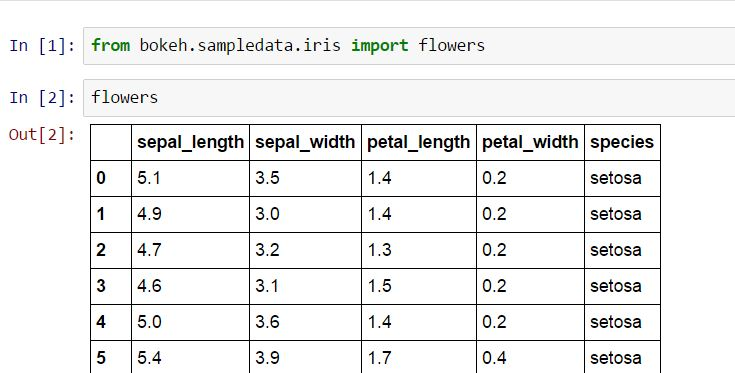
\includegraphics[width=0.8\linewidth]{images/iris-head}
\end{figure}
\begin{framed}
	\begin{verbatim}
	from bokeh.sampledata.iris import flowers
	from bokeh.plotting import figure, show, output_file
	
	colormap = {'setosa': 'red', 
	'versicolor': 'green', 
	'virginica': 'blue'}
	flowers['color'] = 
	flowers['species'].map(lambda x: colormap[x])
	
	output_file("iris.html", 
	title="iris.py example")
	
	p = figure(title = "Iris Morphology")
	p.xaxis.axis_label = 'Petal Length'
	p.yaxis.axis_label = 'Petal Width'
	
	p.circle(flowers["petal_length"],
	flowers["petal_width"],
	color=flowers["color"], 
	fill_alpha=0.2, size=10, )
	show(p)
	\end{verbatim}
\end{framed}
\newpage
\begin{figure}[h!]
	\centering
	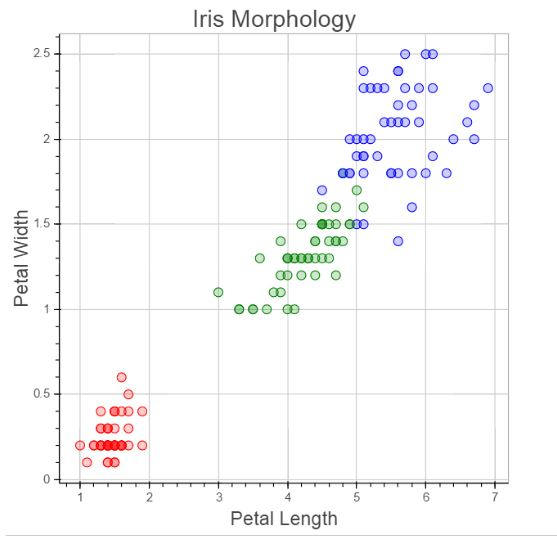
\includegraphics[width=0.6\linewidth]{images/02-iris-scatterplot1-petal}
	
\end{figure}
\subsection*{Exercises}
\begin{itemize}
	\item Try this plot out for different combinations
	of predictors variables.
	\item Try out some different colour combinations for the \texttt{colormap}.
	\item Try this out with a different data set : autompg. (\textit{See the graphic below.})  You can use \texttt{cyl} and \texttt{origin} as grouping variables. \begin{itemize}\item[$\ast$] The levels of cyl are 4,6 and 8. \item[$\ast$] The levels of origin are 1,2 and 3.
	\end{itemize}
\end{itemize}
\begin{figure}[h!]
	\centering
	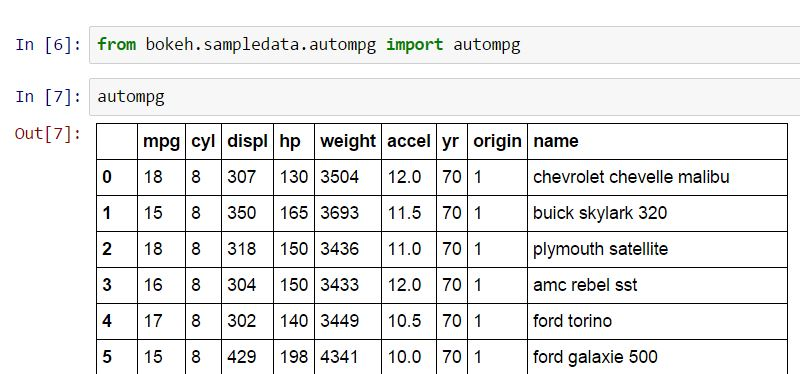
\includegraphics[width=0.9\linewidth]{images/autompg}
\end{figure}

\newpage
\section*{Other interfaces}
\begin{itemize}
	
	\item Bokeh provides some level of Matplotlib compatibility, by using the third-party mplexporter library. 
	\item Although it does not provide 100\% coverage of Matplotlib capabilities, it is still quite useful. 
	\item For instance, in addition to many Matplotlib plots, it is often possible to convert plots created using the python Seaborn and \texttt{ggplot.py} libraries into Bokeh plots very easily. \item Here is a quick example that shows a Seaborn plot converted to a Bokeh plot with just one additional line of code:
\end{itemize}
\newpage

\begin{verbatim}
import seaborn as sns

from bokeh import mpl
from bokeh.plotting import output_file, show

tips = sns.load_dataset("tips")

sns.set_style("whitegrid")

ax = sns.violinplot(x="day", y="total_bill", 
hue="sex",
data=tips, palette="Set2", 
split=True,
scale="count", inner="stick")

output_file("violin.html")

show(mpl.to_bokeh())

\end{verbatim}
\newpage

\section*{Using Palettes}
\begin{itemize}
	\item Palettes are sequences (lists or tuples) of RGB(A) hex strings that define a colormap and be can set as the palette attribute of all chart types from \texttt{bokeh.charts} and as the color attribute of many plot objects from \texttt{bokeh.plotting}. 
	\item Bokeh offers many of the standard Brewer palettes, which can be imported from the \texttt{bokeh.palettes} module. 
	\item For example, importing “\texttt{Spectral6}” gives a six element list of RBG(A) hex strings from the Brewer “Spectral” colormap.
\end{itemize}

\begin{figure}[h!]
	\centering
	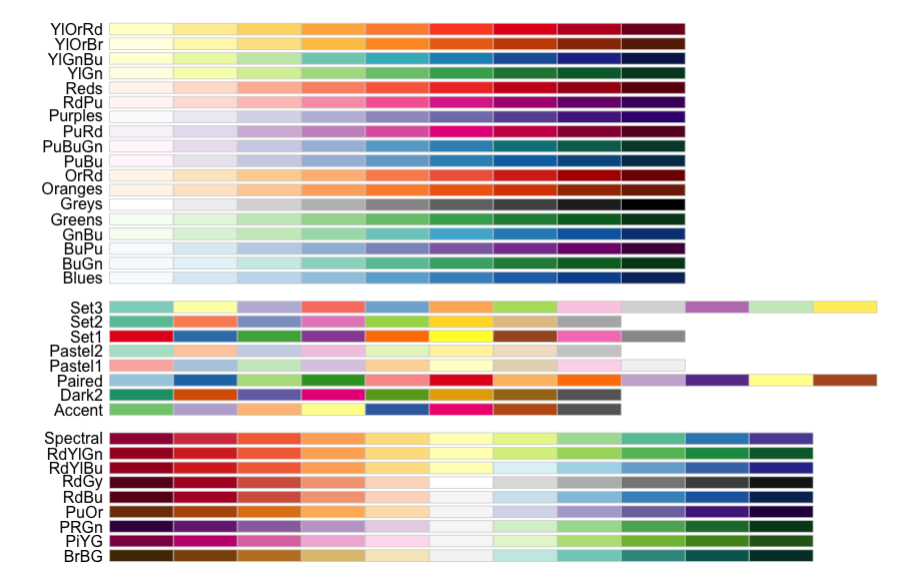
\includegraphics[width=1.2\linewidth]{images/04-pallettes-brewer}
	
\end{figure}

\newpage

{
	\large
	\begin{framed}
		\begin{verbatim}
		>>> from bokeh.palettes import Spectral6
		>>> Spectral6
		[ '#3288bd', '#99d594', '#e6f598', 
		'#fee08b', '#fc8d59', '#d53e4f']
		
		\end{verbatim}
	\end{framed}
}
\begin{itemize}
	\item All of the standard palettes included in bokeh can be found at Standard Palettes.
	\item  Custom palettes can be made by creating sequences of RGB(A) hex strings.
\end{itemize}

%============================================= %

\subsection*{Colourblind Friendly Palettes} The default Palettes, that are used by high level charts,  contain red and green are inappropriate for any colourblind users.
{
	\large
	\begin{framed}
		\begin{verbatim}
		
		from bokeh.palettes import brewer
		palette = brewer["Blues"][3]
		\end{verbatim}
	\end{framed}
}
pass palette into chart call e.g.

{
	\large
	\begin{framed}
		\begin{verbatim}
		
		bar = Bar(medals, countries, title="grouped, dict_input", 
		xlabel="countries", 
		ylabel="medals", 
		legend=True, width=800, height=600, 
		notebook=True, palette=palette)
		\end{verbatim}
	\end{framed}
}
\noindent Palette can actually be a list of any values you want, but there's inbuilt palettes listed in the Bokeh documentation. %http://bokeh.pydata.org/en/latest/docs/reference/palettes.html

\newpage

\section*{Glossary}
In order to make the best use of this User Guide, it is important to have context for some high level concepts and terms. Here is a small glossary of some of the most important concepts in Bokeh.

\subsection*{BokehJS}
The JavaScript client library that actually renders the visuals and handles the UI interactions for Bokeh plots and widgets in the browser. Typically, users will not have to think about this aspect of Bokeh much (“We write the JavaScript, so you don’t have to!”) but it is good to have basic knowledge of this dichotomy. For full details, see the BokehJS chapter of the Developer Guide.
\subsection*{Charts}
Schematic statistical plots such as bar charts, horizon plots, time series, etc. that may include faceting, grouping, or stacking based on the structure of the data. Bokeh provides a high level bokeh.charts interface to quickly construct these kinds of plots. See Using High-level Charts for examples and usage.
\subsection*{Embedding}
Various methods of including Bokeh plots and widgets into web apps and pages, or the IPython notebook. 
% See Embedding Bokeh Plots for more details.
\subsection*{Glyphs}
The basic visual building blocks of Bokeh plots, e.g. lines, rectangles, squares, wedges, patches, etc. The \texttt{bokeh.plotting} interface provides a convenient way to create plots centered around glyphs. 
% See Plotting with Basic Glyphs for more information.
\subsection*{Models}
The lowest-level objects that comprise Bokeh “scenegraphs”. These live in the \texttt{bokeh.models} interface. Most users will not use this level of interface to assemble plots directly. 

However, ultimately all Bokeh plots consist of collections of models, so it is important to understand them enough to configure their attributes and properties. 
% See Styling Visual Attributes for more information.

\subsection*{Server}
The bokeh-server is an optional component that can be used for sharing and publishing Bokeh plots and apps, for handling streaming of large data sets, or for enabling sophisticated user interactions based off of widgets and selections. 
% See Deploying the Bokeh Server for more explanation.

\subsection*{Widgets}
User interface elements outside of a Bokeh plot such as sliders, drop down menus, buttons, etc. Events and updates from widgets can inform additional computations, or cause Bokeh plots to update.
% See Adding Interactions for examples and information.


\end{document}